% !TeX document-id = {9fe05573-0d66-48b0-a749-e436b3eb22be}
%!TeX TXS-program:compile = txs:///xelatex/
\documentclass{beamer}
\usetheme{Darmstadt}

\newif\ifproposal
\proposalfalse

\usepackage{standalone}

\usepackage{CJKutf8}

\usepackage[utf8]{inputenc}
\usepackage[OT1, T2A]{fontenc}
\usepackage{fontspec}
\setmainfont[ItalicFont={*},ItalicFeatures={FakeSlant=.167}]{D2Coding}

\usepackage[normalem]{ulem}
\usepackage{mathtools}
\usepackage{graphicx}
\usepackage{tikz}
%\usetikzlibrary{quantikz}
\usepackage{braket}
\newcommand{\iu}{{i\mkern1mu}}

% based on the original definitions in beamerbasenavigation.sty
\makeatletter
\def\sectionentry#1#2#3#4#5{% section number, section title, page
    %
    \newcount\mymin%
    \mymin=3
    \ifnum\c@section=1%
    \mymin=5
    \fi%
    \ifnum\c@section=2%
    \mymin=4
    \fi%
    %
    \newcount\mymax%
    \mymax=3
    \ifnum\c@section=\beamer@sectionmax%
    \mymax=5
    \fi%
    \ifnum\c@section=\numexpr\beamer@sectionmax-1%
    \mymax=4
    \fi%
    %
    \ifnum\numexpr\c@section-#1<\mymax%
    \ifnum\numexpr#1-\c@section<\mymin%
    \ifnum#5=\c@part%
    \beamer@section@set@min@width
    \box\beamer@sectionbox\hskip1.875ex plus 1fill%
    \beamer@xpos=0\relax%
    \beamer@ypos=1\relax%
    \setbox\beamer@sectionbox=
    \hbox{
        \def\insertsectionhead{#2}%
        \def\insertsectionheadnumber{#1}%
        \def\insertpartheadnumber{#5}%

        {%
            \usebeamerfont{section in head/foot}\usebeamercolor[fg]{section in head/foot}%
            \ifnum\c@section=#1%
            \hyperlink{Navigation#3}{{\usebeamertemplate{section in head/foot}}}%
            \else%
            \hyperlink{Navigation#3}{{\usebeamertemplate{section in head/foot shaded}}}%
            \fi%
        }%
    }%
    \ht\beamer@sectionbox=1.875ex%
    \dp\beamer@sectionbox=0.75ex%
    \fi%
    \fi%
    \fi%
    \ignorespaces%
}

\def\slideentry#1#2#3#4#5#6{%
    %section number, subsection number, slide number, first/last frame, page number, part number
    %
    \newcount\mymin%
    \mymin=3
    \ifnum\c@section=1%
    \mymin=5
    \fi%
    \ifnum\c@section=2%
    \mymin=4
    \fi%
    %
    \newcount\mymax%
    \mymax=3
    \ifnum\c@section=\beamer@sectionmax%
    \mymax=5
    \fi%
    \ifnum\c@section=\numexpr\beamer@sectionmax-1%
    \mymax=4
    \fi%
    %
    \ifnum\numexpr\c@section-#1<\mymax%
    \ifnum\numexpr#1-\c@section<\mymin%
    \ifnum#6=\c@part\ifnum#2>0\ifnum#3>0%
    \ifbeamer@compress%
    \advance\beamer@xpos by1\relax%
    \else%
    \beamer@xpos=#3\relax%
    \beamer@ypos=#2\relax%
    \fi%
    \hbox to 0pt{%
        \beamer@tempdim=-\beamer@vboxoffset%
        \advance\beamer@tempdim by-\beamer@boxsize%
        \multiply\beamer@tempdim by\beamer@ypos%
        \advance\beamer@tempdim by -.05cm%
        \raise\beamer@tempdim\hbox{%
            \beamer@tempdim=\beamer@boxsize%
            \multiply\beamer@tempdim by\beamer@xpos%
            \advance\beamer@tempdim by -\beamer@boxsize%
            \advance\beamer@tempdim by 1pt%
            \kern\beamer@tempdim
            \global\beamer@section@min@dim\beamer@tempdim
            \hbox{\beamer@link(#4){%
                    \usebeamerfont{mini frame}%
                    \ifnum\c@section=#1%
                    \ifnum\c@subsection=#2%
                    \usebeamercolor[fg]{mini frame}%
                    \ifnum\c@subsectionslide=#3%
                    \usebeamertemplate{mini frame}%\beamer@minislidehilight%
                    \else%
                    \usebeamertemplate{mini frame in current subsection}%\beamer@minisliderowhilight%
                    \fi%
                    \else%
                    \usebeamercolor{mini frame}%
                    %\color{fg!50!bg}%
                    \usebeamertemplate{mini frame in other subsection}%\beamer@minislide%
                    \fi%
                    \else%
                    \usebeamercolor{mini frame}%
                    %\color{fg!50!bg}%
                    \usebeamertemplate{mini frame in other subsection}%\beamer@minislide%
                    \fi%
        }}}\hskip-10cm plus 1fil%
    }\fi\fi%
    \else%
    \fakeslideentry{#1}{#2}{#3}{#4}{#5}{#6}%
    \fi%
    \fi%
    \fi%
    \ignorespaces%
}
\makeatother

\AtBeginSection[]{
    \begin{frame}
        \vfill
        \centering
        \begin{beamercolorbox}[sep=8pt,center,shadow=true,rounded=true]{title}
            \usebeamerfont{title}\insertsectionhead\par%
        \end{beamercolorbox}
        \vfill
    \end{frame}
}

\usepackage{xcolor}
\usepackage{pgfplots}
\usepackage{tikz}

\setbeamertemplate{bibliography entry title}{}
\setbeamertemplate{bibliography entry location}{}
\setbeamertemplate{bibliography entry note}{}

% Define bar chart colors
%
\definecolor{bblue}{HTML}{4F81BD}
\definecolor{rred}{HTML}{C0504D}
\definecolor{ggreen}{HTML}{9BBB59}
\definecolor{ppurple}{HTML}{9F4C7C}


\title{Optimizing Quantum Oracle for Standard Hash Algorithms}
%\subtitle{Week 7 Report for Class 75}

\author{Korea University\\Sangheon Lee, Mingyu Cho}

\date{\today}

\newcommand{\shat}[1]{\skew{4.5}\hat{#1}}
\newcommand{\sshat}[1]{\skew{-1.5}\hat{#1}}

\begin{document}
    \begin{frame}
        \titlepage
    \end{frame}

    \begin{frame}
        \frametitle{Table of Contents}
        \tableofcontents
    \end{frame}
    
    \section{Introduction}
    \begin{frame}{Previous Work}
        \begin{itemize}
            \item Studied the basics of quantum computing and Grover's Algorithm
            \item Analysis of reversible quantum S-DES oracle and its construction
            \item Implementation of quantum S-DES oracle with Grover's Algorithm in Microsoft Q\#
        \end{itemize}
    \end{frame}
    
    \begin{frame}{Motivation}
        % why SHA-2/3? why preimage attack (or collision attack, nvm)
        \begin{itemize}
          \item Targeting SHA-2/3
          \begin{itemize}
            \item Current de facto standard hash algorithm
          \end{itemize}
          \item Goal is to perform a preimage attack.
          \begin{itemize}
            \item The most straightforward to apply Grover's Algorithm.
            \item It will be assumed that Grover's Algorithm(or some variation of it) will be applied
            \item Therefore target is to optimize the quantum oracle for SHA-2/3.
          \end{itemize}
        \end{itemize}
    \end{frame}
    
    \begin{frame}{Recap: Grover's Algorithm}
        \begin{itemize}
            \item Searching in an unordered database among $2^n$ elements takes $\tilde{\mathcal{O}}(2^{n/2})$ time complexity and $\tilde{\mathcal{O}}(n)$ quantum space complexity
            \item Proved to be optimal in general
            \item Specifically, improved Grover's Algorithm for collision search yields $\tilde{\mathcal{O}}(2^{n/3})$ time complexity and (quantum) space complexity \cite{brassard1998quantum}
            \begin{itemize}
                \item However, quantum queries are costly in this algorithm
            \end{itemize}
        \end{itemize}
    \end{frame}
    
    \begin{frame}{Chailloux's Algorithm \cite{chailloux2017efficient}}
        \begin{itemize}
            \item Use poly-time qubits and reduce time complexity to $\tilde{\mathcal{O}}(2^{2n/5})$ for collision search and $\tilde{\mathcal{O}}(2^{3n/7})$ for multi-target preimage attacks with additional classic memory
        \end{itemize}
    \end{frame}
    
    \begin{frame}{SHA-2/3 Pre-image Attack Cost Estimation \cite{amy2016estimating}}
        \begin{itemize}
            \item Suggest cost metric for quantum computation based on surface code
            \item Theoretically implement reversible SHA-2/3 quantum circuits
            \item Estimate required physical resources and its scale
        \end{itemize}
    \end{frame}
    
    \begin{frame}{Expectations}
      \begin{itemize}
        \item Focus on micro-scale improvement(regarding quantum oracle)
        \item May be able to reduce the cost in at least one of the following metrics:
          \begin{itemize}
            \item The cost metric from before
            \item The raw number of gates
            \item The number of levels after achieving parallelization
          \end{itemize}
        \item Main target will be the cost metric, not the gates or the levels
      \end{itemize}
    \end{frame}
    
    \begin{frame}{In-depth Topics}
        \begin{itemize}
            \item Surface code(Toric code) : topological quantum error correcting code
            \item Cost metric based on surface code
            \item T-par \cite{amy2014polynomial} : an quantum circuit optimization tool
            \item Advanced quantum circuit (in-place adder, \textit{etc}.)
        \end{itemize}
    \end{frame}
    
    \section{Surface Code}
    \documentclass{beamer}
\usetheme{Darmstadt}
\usepackage{CJKutf8}

\usepackage[utf8]{inputenc}
\usepackage[OT1, T2A]{fontenc}
\usepackage{fontspec}
\usepackage[normalem]{ulem}

\usepackage{graphicx}
\usepackage{tikz}
\usepackage{braket}

\usepackage{xcolor}
\usepackage{pgfplots}
\usepackage{tikz}

\begin{document}

    \subsection{Background}
    \begin{frame}{Surface code and physical qubits}
        This summary is heavily based on \cite{Fowler_2012}.
        \begin{itemize}
            \item Surface code is a method to construct \textit{logical} qubits from physical qubits with acceptable relativce error tolerance \cite{calderbank1997quantum}
            \item Logical qubits are more efficient than their physical counterparts
            \item The tolerance of surface codes to errors is high as about 1\%
            \item However, ensuring high tolerance requires massive physical qubits and sequential Toffoli gates
            \begin{itemize}
                \item ``We assume an error rate approximately one-tenth the threshold rate, which implies that we need about 14,500 physical qubits per logical qubit to give a sufficiently low logical error rate to successfully execute the algorithm"
            \end{itemize}
        \end{itemize}
    \end{frame}
    
    \begin{frame}{Surface code and physical qubits}
        \begin{itemize}
            \item However, ensuring high tolerance requires massive physical qubits and sequential Toffoli gates
            \begin{itemize}
                \item ``A much larger part of the surface code is however needed to generate and purify the special ancilla $\ket{A_L}$ states that are used in the Toffoli gates.""
                \item Applying Shor's Algorithm to 2,000-bit integer requires $ 2.2 \times 10^{12} \ket{A_L}$ states and takes about 26.7 hours
                \item The surface code needs to generate these states in a timely manner
            \end{itemize}
        \end{itemize}
    \end{frame}
    
    \begin{frame}{Surface code and physical qubits}
        \begin{itemize}
            \item However, ensuring high tolerance requires massive physical qubits and sequential Toffoli gates
            \begin{itemize}
                \item ``We assume an error rate approximately one-tenth the threshold rate, which implies that we need about 14,500 physical qubits per logical qubit to give a sufficiently low logical error rate to successfully execute the algorithm"
                \item In result, 58 million qubits are required for computation
                \item Additionally 1 billion qubits are required for generating $\ket{A_L}$ states
            \end{itemize}
            \item Hopefully, ``the size of the quantum computer is quite sensitive tothe error rate in the physical qubits.''
            \begin{itemize}
                \item ``For example, improving the overall error rate by about a factor of ten, as detailed in Appendix M, can reduce the number of physical qubits by about an order of magnitude, to about 130 million, although leaving the execution time unchanged.''
            \end{itemize} 
        \end{itemize}
    \end{frame}
    
    \subsection{Introduction}
    \begin{frame}{Introduction: Qubit operators}
        Quantum computation is based on qubits: two-level quantum systems
        \begin{itemize}
            \item Based on quantum physics and election spins
        \end{itemize}
        These electron spins can be reprensented by various operators such as Pauli-X, Y, Z operators.
    \end{frame} 
           
    \begin{frame}{Qubit operators}
        Basic recap of Pauli operators and qubit operators:
        \begin{itemize}
            \item Ground state for $\shat{Z}$ axis : $\ket{g} = \begin{pmatrix} 1 \\ 0 \end{pmatrix}$
            \item Excited state : $\ket{e} = \begin{pmatrix} 0 \\ 1 \end{pmatrix}$
            \item $\shat{Z} = \hat{\sigma_z} = \begin{pmatrix}
            1 & 0 \\
            0 & -1
            \end{pmatrix}$, with eigenvalues $+1$ and $-1$ for $\ket{g}$, $ \ket{e} $.
            \item $\shat{X} = \hat{\sigma_x} = \begin{pmatrix}
            0 & 1 \\
            1 & 0
            \end{pmatrix}$, with eigenvalues $+1$ and $-1$ for $\ket{+} = \frac{1}{\sqrt{2}}\begin{psmallmatrix} 1 \\ 1 \end{psmallmatrix} = \frac{1}{\sqrt{2}}(\ket{g} + \ket{e})$, $\ket{-} = \frac{1}{\sqrt{2}}\begin{psmallmatrix} 1 \\ -1 \end{psmallmatrix} = \frac{1}{\sqrt{2}}(\ket{g} - \ket{e})$.
            \item $\shat{Y} = -i\hat{\sigma_y} = \shat{Z}\shat{X} = \begin{pmatrix}
            0 & 1 \\
            -1 & 0
            \end{pmatrix}$, which is real unlike $ \hat{\sigma_y} $.
        \end{itemize}
    \end{frame}
    
    \begin{frame}{Qubit operators}
        These qubit operators satisfy the following:
        \begin{equation}
        \begin{split}
            \shat{X}^2 &= -\shat{Y}^2 = \shat{Z}^2 = I \\
            \shat{X}\shat{Z} &= -\shat{Z}\shat{X} \\
            [\shat{X},\shat{Y}] &= \shat{X}\shat{Y} - \shat{Y}\shat{X} = -2\shat{Z}
        \end{split}
        \end{equation}
        Also note that each measurement based on each quantum operators yields one of its eigenstates. For example, $M_Z$ will return $ \ket{g} $ or $ \ket{e} $, while $ M_X $ will return $ \ket{+} $ or $ \ket{-} $.
    \end{frame} 

    \begin{frame}{Single-qubit errors}
        Qubits errors are random $ \shat{X} $ bit-flip and/or $ \shat{Z} $ phase-flip.
        \begin{itemize}
            \item These single-qubit errors can be undone after detection
            \begin{itemize}
                \item Erroneous $ \shat{Z} $ can be cancelled with another $ \shat{Z} $ since $ \shat{Z}^2 = I $
            \end{itemize}
            \item Also, applying qubit operation does not alter the probability of its eigenstate
        \end{itemize}
        Thus detection, rather than correction, is the key point of surface code.
    \end{frame}
    
    \begin{frame}{Single-qubit errors}
        \begin{itemize}
            \item However since $ [\shat{X}, \shat{Z}] \neq \hat{0} $, sequential measurements of $ \shat{X} $ and $ \shat{Z} $ might conflict each other (since $ \shat{X}\shat{Z} \neq \shat{Z}\shat{X} $).
            \item This problem can be avoided by measuring multi-qubits at once. Consider qubit $ a $ and $ b $ and operation $ \sshat{X_a}\sshat{X_b} $ and $ \sshat{Z_a}\sshat{Z_b} $, then these two operations do commute!
        \end{itemize}
        \begin{equation}
        \begin{split}
        [\sshat{X_a}\sshat{X_b}, \sshat{Z_a}\sshat{Z_b}] &= (\sshat{X_a}\sshat{X_b})(\sshat{Z_a}\sshat{Z_b}) - (\sshat{Z_a}\sshat{Z_b})(\sshat{X_a}\sshat{X_b}) \\
        &= \sshat{X_a}\sshat{Z_a}\sshat{X_b}\sshat{Z_b} - \sshat{Z_a}\sshat{X_a}\sshat{Z_b}\sshat{X_b} \\
        &= (-\sshat{Z_a}\sshat{X_a})(-\sshat{Z_b}\sshat{X_b}) - (\sshat{Z_a}\sshat{X_a})(\sshat{Z_b}\sshat{X_b}) \\
        &= \hat{0}
        \end{split}
        \end{equation}
    \end{frame}
    

\end{document}
    
    \section{Clifford + T gate}
    \begin{frame}{Why Clifford + T?}
    	\begin{itemize}
    		\item By Gottesman-Knill Theorem, Clifford gates can be simulated efficiently on a classical computer.
    		\item T-gate is eqal to $R_{\pi/4}=\begin{pmatrix}1 & 0 \\ 0 & \sqrt{i}\end{pmatrix}$, a $\frac{\pi}{4}$ rotation.
    		\item Clifford+T gate utilizes only one inefficient gate, while is universal.
    	\end{itemize}
    \end{frame}
    
    \section{Ripple-Carry Adder}
    \begin{frame}
      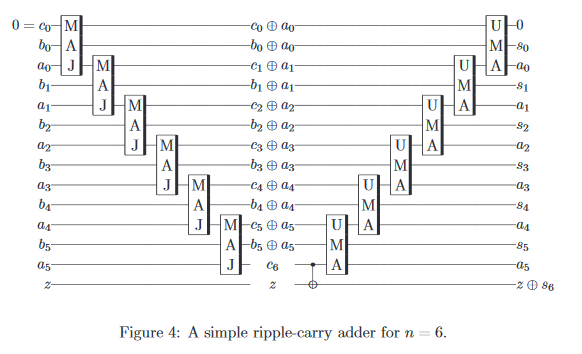
\includegraphics[width=\textwidth]{./Images/ripple-carry-adder.jpg}
    \end{frame}
  	
  	\section{}
    
    \section{References}
    \begin{frame}[allowframebreaks]
        \frametitle{References}
        \bibliographystyle{amsalpha}
        \bibliography{./quantum.bib}
    \end{frame}
\end{document}